\documentclass[t, screen, aspectratio=43]{beamer}
\usepackage[T1]{fontenc}
\usepackage[utf8]{inputenc}
\usepackage{epsf}
\usepackage{graphicx}
\usepackage{geometry}
\usepackage{tabularx}
\usepackage[table]{colortbl}
\usepackage{xcolor}
\usepackage{soul}
\usepackage[normalem]{ulem}
\usepackage{tikz}
\usepackage{subcaption}
\usepackage{hyperref}
\usepackage{skak}
% Use the NTNU-temaet for beamer 
% \usetheme[style=ntnu|simple|vertical|horizontal, 
%     language=bm|nn|en, 
%     smalltitle, 
%     city=all|trondheim|alesund|gjovik]{ntnu2017}
\usetheme[style=helvet,language=en]{ntnu2017}

\usepackage[english]{babel}
\usepackage[style=numeric,backend=biber,natbib=false,sorting=none]{biblatex}

\title[Short title]{Ultra low power integer-N ADPLL}
\subtitle{Master's thesis project - meeting 6}
\author[C Nielsen]{Cole Nielsen}
\institute[NTNU]{Department of Electronic Systems, NTNU}
\date{21 February 2020 \symking (calendar week 8)}
%\date{} % To have an empty date

\addbibresource{example.bib} % Add bibliography database

% Set the reference style to numeric.
% See here: http://tex.stackexchange.com/questions/68080/beamer-bibliography-icon
\setbeamertemplate{bibliography item}[text] 

% Set bibliography fonts to a small size.
\renewcommand*{\bibfont}{\footnotesize}

\usepackage{tikz}
\usepackage{enumitem}
\newcommand*\mycirc[1]{%
\begin{tikzpicture}[baseline=(C.base)]
	\node[draw,circle,inner sep=1pt,minimum size=3ex](C){#1};
\end{tikzpicture}}


\begin{document}

\begin{frame}
	\titlepage%
\end{frame}

% Alternatively, special title page command to get a different background
% \ntnutitlepage

% #############################################################################
% This week
% #############################################################################

\begin{frame}
	\frametitle{Overview}
	\begin{block}{For this week...}
		\begin{enumerate}[itemsep=4pt,label=\protect\mycirc{\arabic*}]
			\scriptsize
			\item Figure out synthesis, place and route with Genus and Innovus
			\item Tested with BBPD, Loop filter
		\end{enumerate} 
	\end{block}	
\end{frame}


% #############################################################################
% This week
% #############################################################################


% #############################################################################
% Physical limits
% #############################################################################


\begin{frame}
	\frametitle{Invecas model}
	\begin{block}{Generating new Invecas models???}
	\tiny
	\begin{itemize}[itemsep=4pt,label=\protect---]
		\item The GF22FDX models used for synthesis (from \texttt{\textbackslash eda\textbackslash kits\textbackslash invecas\textbackslash ...}) have sort of odd voltages defined, i.e. $V_{dd}$ = \{0.59, 0.65\}, body bias = \{0.45, 0.8\} for TT corner. 
		\item Also, only SLVT is available.
		\item These library files say they are generated from Cadence Liberate, is this something I can also use to generate new .lib files with $V_{dd}$/body bias closer to my needs?
	\end{itemize}
	% \vspace{-3em}

	\end{block}	

	\begin{figure}[htb!]
	    \centering
	    \begin{subfigure}{0.6\textwidth}
	        \centering
	        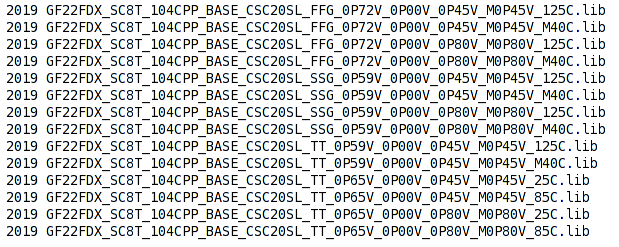
\includegraphics[width=1\textwidth, angle=0]{invecas_model_names.png}
	    \end{subfigure}%
	    \begin{subfigure}{0.4\textwidth}
	        \centering
	        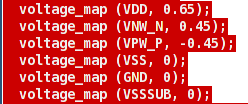
\includegraphics[width=0.6\textwidth, angle=0]{invecas_model.png}
	    \end{subfigure}
	    % \caption{Approximate model for ring oscillator inverter delay cell.}
	\end{figure}

\end{frame}


\begin{frame}
	\frametitle{Synthesis/place and route}
	\begin{block}{Attempt 1: BBPD.}
	\tiny
	\begin{itemize}[itemsep=4pt,label=\protect---]
		\item Tried simple test first...

	\end{itemize}
	% \vspace{-3em}
	\begin{figure}[htb!]
	    \centering
	    \begin{subfigure}{0.5\textwidth}
	        \centering
	        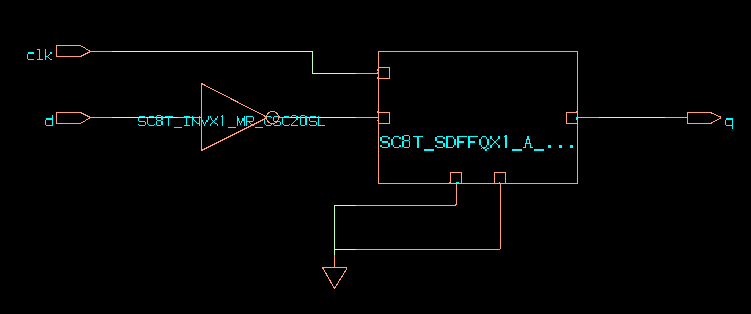
\includegraphics[width=0.8\textwidth, angle=0]{bbpd_synth_schem.png}
	    \end{subfigure}%
	    \begin{subfigure}{0.5\textwidth}
	        \centering
	        \center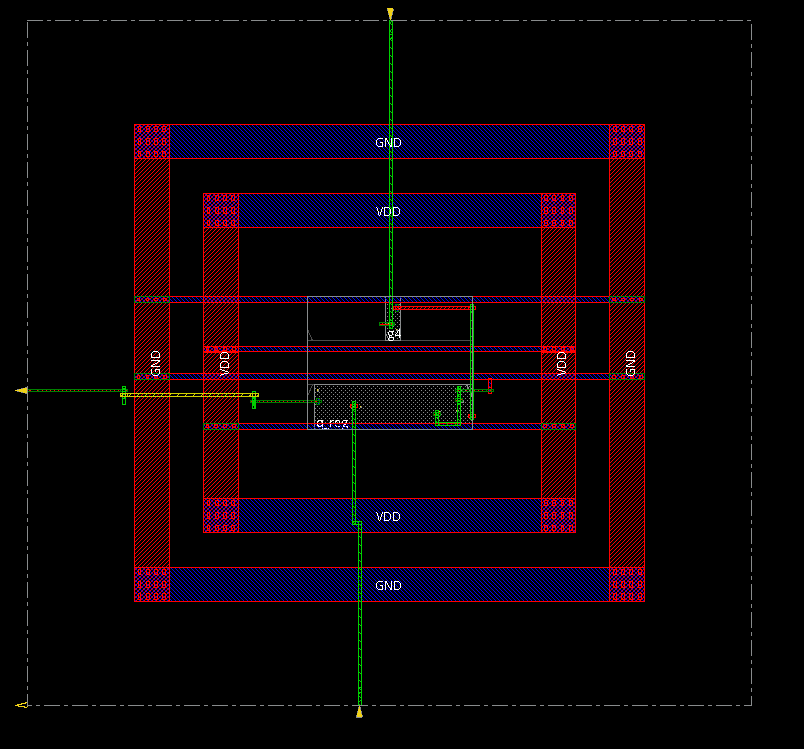
\includegraphics[width=0.8\textwidth, angle=0]{bbpd_pnr.png}
	    \end{subfigure}
	    % \caption{Approximate model for ring oscillator inverter delay cell.}
	\end{figure}

	\end{block}	
\end{frame}

\begin{frame}
	\frametitle{Synthesis/place and route}
	\begin{block}{Loop filter}
	\tiny
	\begin{itemize}[itemsep=4pt,label=\protect---]
		\item Constructed using 16 bit width for all parts of datapath (3x adders, 4x multipliers).
	\end{itemize}
	% \vspace{-3em}
	\begin{figure}[htb!]
	        \centering
	        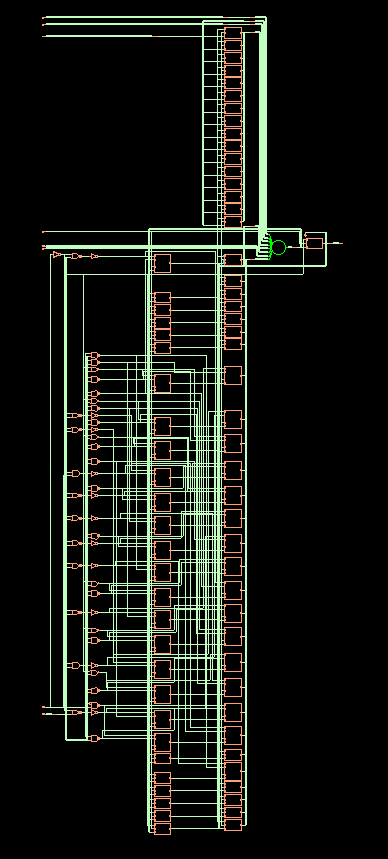
\includegraphics[width=0.3\textwidth, angle=90]{lf_schem}
	    % \caption{Approximate model for ring oscillator inverter delay cell.}
	\end{figure}

	\end{block}	
\end{frame}


\begin{frame}
	\frametitle{Synthesis/place and route}
	\begin{block}{Power estimate}
	\tiny
	\begin{itemize}[itemsep=4pt,label=\protect---]
		\item 117.6 $\mu$W with $V_{DD}$ = 0.65, 0.45V body bias, TT corner, 25C.
		\item Probably is lower if I reduce the supply (0.5V?). 
		\item Can reduce the design to PI controller only, removed 2 multipliers (should reduce power $\sim$2x?)
	\end{itemize}
	\vspace{-1em}
	\begin{figure}[htb!]
	        \centering
	        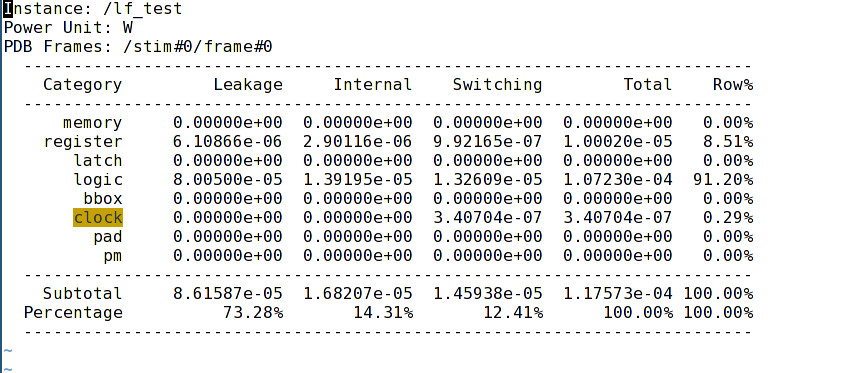
\includegraphics[width=1\textwidth, angle=0]{lf_power}
	    % \caption{Approximate model for ring oscillator inverter delay cell.}
	\end{figure}

	\end{block}	
\end{frame}


\begin{frame}
	\frametitle{Synthesis/place and route}
	\begin{block}{Area estimate}
	\tiny
	\begin{itemize}[itemsep=4pt,label=\protect---]
		\item Area of 1891 $\mu$m$^2$. Equal to 43.5x43.5 $\mu$m
	\end{itemize}
	\vspace{-1em}
	\begin{figure}[htb!]
	        \centering
	        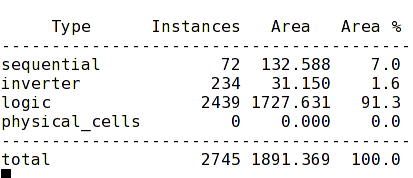
\includegraphics[width=0.8\textwidth, angle=0]{lf_area}
	    % \caption{Approximate model for ring oscillator inverter delay cell.}
	\end{figure}

	\end{block}	
\end{frame}

\begin{frame}
	\frametitle{\color{red}Original estimates...}
	\begin{block}{Component-level specs}
		\scriptsize
		\begin{itemize}[itemsep=4pt,label=\protect---]
			\scriptsize
			\item Given 22-FDX yields ca. 5.5 MGates/mm$^2$, assume $\alpha$ = 0.1, $f_{clk}$ = 16 MHz:
		\end{itemize} 
	\vspace{-1em}
	\begin{table}[h!]
		\centering
		\def\arraystretch{1.5}		
		\setlength\arrayrulewidth{0.75pt}
		\setlength{\tabcolsep}{1em} % for the horizontal padding
		\tiny
		\begin{tabular}{|c|c|c|c|c|}
			\hline 
			\rule[-1ex]{0pt}{2.5ex} \cellcolor{gray!40}\textbf{Datapath bits} & \cellcolor{gray!40}\textbf{Gates+DFFs} & \cellcolor{gray!40}\textbf{Area} [$\mu m^2$] & \cellcolor{gray!40}\textbf{Square side [$\mu m$]} &  \cellcolor{gray!40}\textbf{Power} [$\mu$W], $\alpha$ = 0.1\\ 
			\hline 
			\rule[-1ex]{0pt}{2.5ex} 8 & 2652 & 521 & 22.8 & 4.24 \\ 
			\hline 
			\rule[-1ex]{0pt}{2.5ex} 9 & 3390 & 660 & 25.7 & 5.42 \\ 
			\hline 
			\rule[-1ex]{0pt}{2.5ex} 10 & 4213 & 815 & 28.5 & 6.74 \\ 
			\hline 
			\rule[-1ex]{0pt}{2.5ex} 11 & 5127 & 986 & 31.4 & 8.20 \\ 
			\hline 
			\rule[-1ex]{0pt}{2.5ex} 12 & 6126 & 1172 & 34.2 & 9.80 \\ 
			\hline 
			\rule[-1ex]{0pt}{2.5ex} 13 & 7216 & 1375 & 37.1 & 11.5 \\ 
			\hline 
			\rule[-1ex]{0pt}{2.5ex} 14 & 8391 & 1594& 39.9 & 13.4 \\ 
			\hline 
			\rule[-1ex]{0pt}{2.5ex} 15 & 9657 & 1829 & 42.8 & 15.5 \\ 
			\hline 
			\rule[-1ex]{0pt}{2.5ex} \cellcolor{yellow}16 & \cellcolor{yellow}11008 & \cellcolor{yellow}2080 & \cellcolor{yellow}45.6 & \cellcolor{yellow}17.6 \\ 
			\hline 
		\end{tabular} 
		% \caption{Assigned specifications for branch line hybrid design.}
		% \label{asgn_specs}
		\label{design_specs}
	\end{table}   
		\scriptsize
		\vspace{-1em}
		\begin{itemize}[itemsep=4pt,label=\protect---]
			\scriptsize
			\item \textbf{Area is close}. Power is off, however it was based on a guess based relative to values obtained at 0.35V.
		\end{itemize} 
	\end{block}    
\end{frame}



\begin{frame}
	\frametitle{Synthesis/place and route}
	\begin{block}{Loop filter layout.}
	\tiny
	\begin{itemize}[itemsep=4pt,label=\protect---]
		\item First iteration at loop filter layout... still need to extract the circuit/LVS etc...
	\end{itemize}
	\vspace{-1em}
	\begin{figure}[htb!]
	        \centering
	        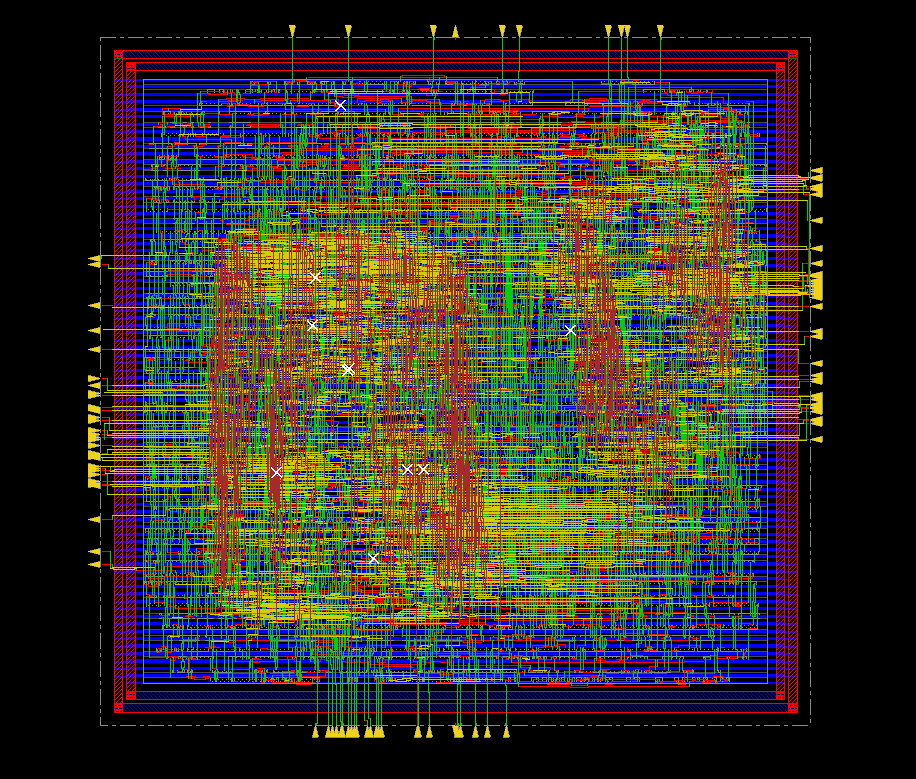
\includegraphics[width=0.5\textwidth, angle=0]{lf_layout}
	    % \caption{Approximate model for ring oscillator inverter delay cell.}
	\end{figure}

	\end{block}	
\end{frame}






% #############################################################################
% Loop Dynamics (continuous)
% #############################################################################

% \begin{frame}
% 	\frametitle{Loop Dynamics}
% 	\begin{block}{Still To Do}
% 		\vspace{-.2em}
% 		\begin{itemize}
% 			\footnotesize
% 			\item Standard approach to used mixed continuous/discrete time mathematical model for DPLL. 
% 			\item Plot of RO phase noise (typical)
% 			\item Automatic analysis of performance (lock detection, residual phase modulation, lock-in/pull-in range).
% 			\item Automatic optimization (using gradient descent) of PLL parameters?
% 			\item Z-domain modeling of loop? Develop (by hand) some ideal transfer funtions for loop.

% 		\end{itemize}    
% 	\end{block}
% \end{frame}

% #############################################################################
% Architecture - block diagram
% #############################################################################


\begin{frame}
	\frametitle{Architecture}
	\begin{block}{Block Diagram}
	\center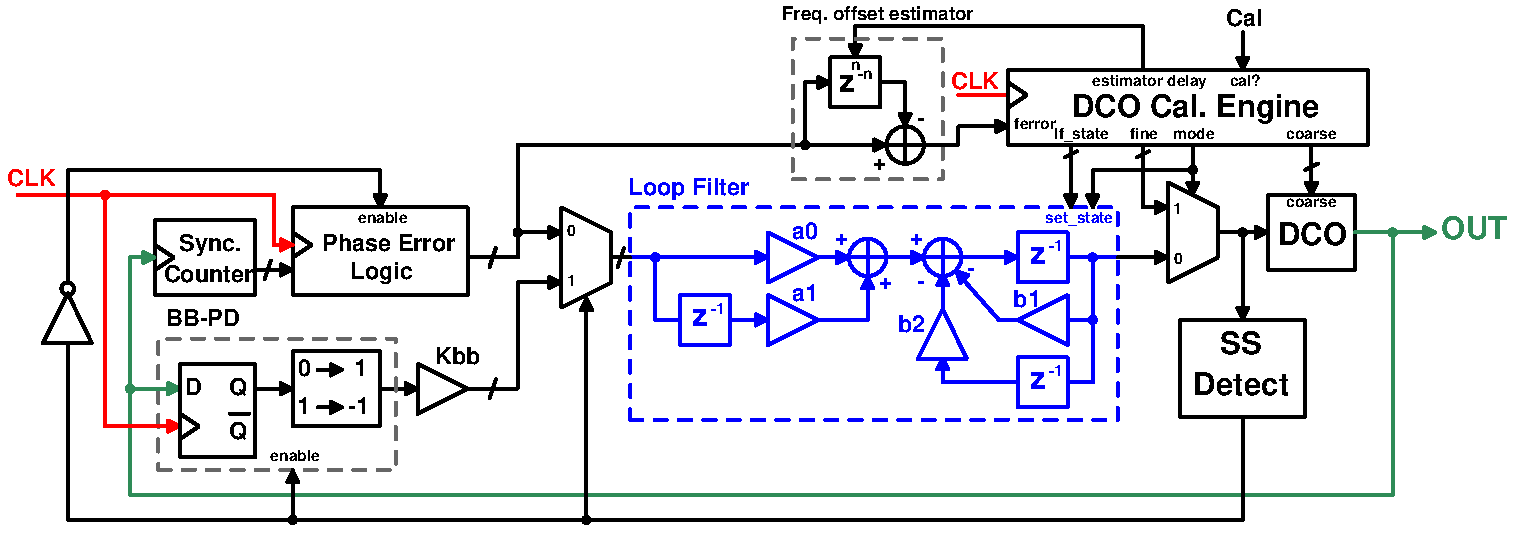
\includegraphics[width=0.8\textwidth, angle=0]{pll_master_arch.pdf}

	\end{block}
		\begin{block}{Power Targets {\color{red}(revised)}}
		\scriptsize
		{\color{red}\textbf{(Divider not necessary)}}
		\vspace{-1em}
		\begin{table}[htb!]
			\tiny
			\centering
			\def\arraystretch{1.5}		
			\setlength\arrayrulewidth{0.75pt}
			\setlength{\tabcolsep}{1em} % for the horizontal padding
			\begin{tabular}{|l|l|l|l|l|l|}
				\hline 
				\rule[-1ex]{0pt}{2.5ex} \cellcolor{gray!40}\textbf{DCO} & \cellcolor{gray!40}\textbf{Phase detector} & \cellcolor{gray!40}\textbf{Divider }& \cellcolor{gray!40}\textbf{Digital (LF)}& \cellcolor{gray!40}\textbf{Other} & \cellcolor{gray!40}\textbf{SUM} \\ 
				\hline 
				\rule[-1ex]{0pt}{2.5ex} 50 $\mu$W& 10 $\mu$W & \textbf{N/A} {\color{red}\st{10 $\mu$W}} & 10 $\mu$W  & $\leq$ \textbf{5} {\color{red}\st{10}} $ \mu$W & $\leq$ \textbf{75} {\color{red}\st{100}} $\mu$W\\ 
				\hline 
			\end{tabular} 
			% \caption{Assigned specifications for branch line hybrid design.}
			% \label{asgn_specs}
		\end{table}   
	\end{block}

\end{frame}

% #############################################################################
% Specification
% #############################################################################

\begin{frame}
	\frametitle{Specification\color{black}}
	\begin{block}{System Performance Targets}
		\tiny
		\begin{table}[h!]
			\centering
			\def\arraystretch{1.5}		
			\setlength\arrayrulewidth{0.75pt}
			\setlength{\tabcolsep}{1em} % for the horizontal padding
			\begin{tabular}{|l|r|l|l|}
				\hline 
				\rule[-1ex]{0pt}{2.5ex} \cellcolor{gray!40}\textbf{Parameter} & \cellcolor{gray!40}\textbf{Value} & \cellcolor{gray!40}\textbf{Unit }& \cellcolor{gray!40}\textbf{Notes}\\ 
				\hline 
				\rule[-1ex]{0pt}{2.5ex} \textbf{Frequency}  & 2.4-2.4835 & GHz & 2.4G ISM Band\\ 
				\hline 
				\rule[-1ex]{0pt}{2.5ex} \textbf{Ref. frequency} & 16 & MHz & Yields 6 channels \\ 
				\hline 
				\rule[-1ex]{0pt}{2.5ex} \textbf{Power} & $\leq$ \textbf{75} {\color{red}\st{100}} $\mu$W  &$\mu$W & Minimize!\\ 
				\hline 
				\rule[-1ex]{0pt}{2.5ex} \textbf{FSK BER} & $\leq$ 1e-2  & & GFSK\textbf{*} with $f_{dev}$=$\pm$250 KHz\\ 
				\hline 
				\rule[-1ex]{0pt}{2.5ex} \textbf{CNR} & $>$ 20 & dBc&Yields  \textbf{-235} {\color{red}\st{-233}} dB FOM$_{jitter}$ ideally \\ 
				\hline 
				\rule[-1ex]{0pt}{2.5ex} \textbf{Initial Lock Time} & $\leq$ 10 & $\mu$s & Upon cold start \\ 
				\hline 
				\rule[-1ex]{0pt}{2.5ex} \textbf{Re-lock Time} & $\leq$ 5 & $\mu$s & Coming out of standby, $f_{error} <$ \textbf{1 MHz} \\ 
				\hline 
				\rule[-1ex]{0pt}{2.5ex} \textbf{Lock $\Delta f$ tolerance} & $100$ & kHz& \\ 
				\hline 
				\rule[-1ex]{0pt}{2.5ex} \textbf{FOM}$_{\textnormal{jitter}}$ & $\leq$ -230 & dB & \textbf{For state of art in size/power} \\ 
				\hline 
				\rule[-1ex]{0pt}{2.5ex} \textbf{Area} & $<$ 0.01  & mm$^2$ & \\ 
				\hline 
			\end{tabular} 
			% \caption{Assigned specifications for branch line hybrid design.}
			% \label{asgn_specs}
		\end{table}   
		\textbf{*} Using BT=0.3, 1 MSymbols/s, 4 demodulated symbols averaged per bit to yield 250 kbps.
	\end{block}    
\end{frame}



\begin{frame}
	\frametitle{Specification\color{black}}
	\begin{block}{Component-level specs}
		\scriptsize
	\begin{table}[h!]
		\centering
		\tiny
		\def\arraystretch{1.5}		
		\setlength\arrayrulewidth{0.75pt}
		\setlength{\tabcolsep}{1em} % for the horizontal padding
		\begin{tabular}{|l|r|l|}
			\hline 
			\rule[-1ex]{0pt}{2.5ex} \cellcolor{gray!40}\textbf{Parameter} & \cellcolor{gray!40}\textbf{Value} & \cellcolor{gray!40}\textbf{Unit }\\ 
			\hline 
			\rule[-1ex]{0pt}{2.5ex} \textbf{Counter range}  & 256 steps & coverage of 150-155 \\ 
			\hline 
			\rule[-1ex]{0pt}{2.5ex} \textbf{Divider ratio} & 150-155  & (For non-counter based)\\ 
			\hline 
			\rule[-1ex]{0pt}{2.5ex} {\color{red}\st{\textbf{TDC resolution}}} &{\color{red}\st{$\geq$ 155}}  & {\color{red}\st{steps/reference cycle}}\\ 
			\hline 
			\rule[-1ex]{0pt}{2.5ex} \textbf{DCO gain $K_{DCO}$} & $10^4$ & Hz/LSB \\ 
			\hline 
			\rule[-1ex]{0pt}{2.5ex} \textbf{DCO tuning range} & 10 & MHz \\ 
			\hline 
			\rule[-1ex]{0pt}{2.5ex} \textbf{DCO DAC resolution} & 10 & bit \\ 
			\hline 
			\rule[-1ex]{0pt}{2.5ex} \textbf{DCO Phase noise} &$<$ -80 & dBc/Hz @ $\Delta f=10^6$ Hz, $f_c$ = 2.448 GHz \\ 
			\hline 
			\rule[-1ex]{0pt}{2.5ex} \textbf{DCO Power} & $\leq$ 50 & $\mu$W \\ 
			\hline 
			\rule[-1ex]{0pt}{2.5ex} \textbf{Digital filter word resolution} & $\leq$ 16 & bits (power grows as $\mathcal{O}(n^2)$) \\ 
			\hline 
			\rule[-1ex]{0pt}{2.5ex} \textbf{BB-PD jitter} & $\leq$ 12 & ps$_{\textnormal{rms}}$ \\ 
			\hline 
		\end{tabular} 
		% \caption{Assigned specifications for branch line hybrid design.}
		% \label{asgn_specs}
		\label{design_specs}
	\end{table}   
	\end{block}    
\end{frame}

% #############################################################################
% Timeline
% #############################################################################

\begin{frame}
	\frametitle{Time plan (pt. 1)}
	\begin{table}[htb!]
		\tiny
		\centering
		\vspace{-1em}
		\def\arraystretch{1.5}		
		\setlength\arrayrulewidth{0.75pt}
		\setlength{\tabcolsep}{1em} % for the horizontal padding
		\begin{tabular}{|c|l|l|l|}
			\hline 
			\rule[-1ex]{0pt}{2.5ex}\cellcolor{gray!40}\textbf{Week \#} & \cellcolor{gray!40}\textbf{Dates} &\cellcolor{gray!40}\textbf{Tasks} & \cellcolor{gray!40}\textbf{Outcomes}\\ 
			\hline 
			% \rule[-1ex]{0pt}{2.5ex} \cellcolor{green!20}\textbf{3}&\cellcolor{green!20}13.1 - 19.1 &\cellcolor{green!20}Review PLL Design &\cellcolor{green!20}Refreshed Knowledge\\ 
			% \hline 
			\rule[-1ex]{0pt}{2.5ex}\cellcolor{red!40}\textbf{4}&\cellcolor{red!40}20.1 - 26.1 &\cellcolor{red!40}Finalize high level modeling &\cellcolor{red!40}Component level specification\\ 
			\hline 
			\rule[-1ex]{0pt}{2.5ex}\textbf{5}\cellcolor{red!40}&\cellcolor{red!40}27.1 - 2.2 &\cellcolor{red!40}Establish test bench in Virtuoso &\cellcolor{red!40}With ideal PLL implementation\\ 
			\hline 
			\rule[-1ex]{0pt}{2.5ex}\cellcolor{red!40}\textbf{6}&\cellcolor{red!40}3.2 - 9.2&\cellcolor{red!40}Schem. design: phase detector &\cellcolor{red!40}TDC - flash and counter based \\ 
			\hline 
			\rule[-1ex]{0pt}{2.5ex}\cellcolor{red!40}\textbf{7}&\cellcolor{red!40}10.2 - 16.2&\cellcolor{red!40}Schem. design: phase detector &\cellcolor{red!40}Bang-bang phase detector\\ 
			\hline 
			\rule[-1ex]{0pt}{2.5ex}\cellcolor{green!40}\textbf{8}&\cellcolor{green!40}17.2 - 23.2&\cellcolor{green!40}RTL, synthesis, place\&route &\cellcolor{green!40}Digital loop filter\\ 
			\hline 
			\rule[-1ex]{0pt}{2.5ex}\textbf{9}&24.2 - 1.3& RTL, synthesis, place\&route & Digital loop filter\\ 
			\hline 
			\rule[-1ex]{0pt}{2.5ex}\textbf{10}&2.3 - 8.3& Schem. design: oscillator & Ring DCO\\ 
			\hline 
			\rule[-1ex]{0pt}{2.5ex}\textbf{11}&9.3 - 15.3& Schem. design: oscillator & LC DCO\\ 
			\hline 
			\rule[-1ex]{0pt}{2.5ex}\textbf{12}&16.3 - 22.3& Schem. design: divider  &TSPC + pulse swallow or sync counter?\\ 
			\hline 
			\rule[-1ex]{0pt}{2.5ex}\textbf{13}&23.3 - 29.3&Schem. design: Calibration& RTL/schem. for calibration\\ 
			\hline 
			\rule[-1ex]{0pt}{2.5ex}\textbf{14}& 30.3 - 5.4 &  Flex week - schem. design & Finalize schematic level design\\ 
			\hline 
			\rule[-1ex]{0pt}{2.5ex}\textbf{15}& 6.4 - 12.4& {\color{red}\textbf{Easter}} & - \\ 
			\hline 
			\rule[-1ex]{0pt}{2.5ex}\textbf{16}& 13.4 - 19.4& Layout & Phase detector\\ 
			\hline 
			\rule[-1ex]{0pt}{2.5ex}\textbf{17}& 20.4 - 26.4& Layout & Oscillator\\ 
			\hline 
		\end{tabular}
		\begin{flushleft}\textbf{Legend:} \colorbox{red!20}{\textbf{Done}} \colorbox{green!20}{\textbf{Current}}  \colorbox{blue!20}{\textbf{Revised}}
		% *I will write the report simultaneously with the work.
		\end{flushleft}
		% \caption{Assigned specifications for branch line hybrid design.}
		% \label{asgn_specs}
	\end{table}   
\end{frame}

\begin{frame}
	\frametitle{Time plan (pt. 2)}
	\begin{table}[htb!]
		\tiny
		\centering
		\vspace{-1em}
		\def\arraystretch{1.5}		
		\setlength\arrayrulewidth{0.75pt}
		\setlength{\tabcolsep}{1em} % for the horizontal padding
		\begin{tabular}{|c|l|l|l|}
			\hline 
			\rule[-1ex]{0pt}{2.5ex}\cellcolor{gray!40}\textbf{Week \#} & \cellcolor{gray!40}\textbf{Dates} &\cellcolor{gray!40}\textbf{Tasks} & \cellcolor{gray!40}\textbf{Outcomes}\\ 
			\hline 
			\rule[-1ex]{0pt}{2.5ex}\textbf{18}& 27.4 - 3.5 & Layout & Divider/calibration\\ 
			\hline 
			\rule[-1ex]{0pt}{2.5ex}\textbf{19}& 4.5 - 10.5 & Layout & Finalization/system integration\\ 
			\hline 
			\rule[-1ex]{0pt}{2.5ex}\textbf{20}& 11.5 - 17.5 & Flex week (layout) OR yield improvement & Depending on progress\\ 
			\hline 
			\rule[-1ex]{0pt}{2.5ex}\textbf{21}& 18.5 - 24.5& {\color{blue}\textbf{Report writing}} & \\ 
			\hline 
			\rule[-1ex]{0pt}{2.5ex}\textbf{22}& 25.5 - 31.5& {\color{blue}\textbf{Report writing}} & \\ 
			\hline 
			\rule[-1ex]{0pt}{2.5ex}\textbf{23}& 1.6 - 7.6& {\color{blue}\textbf{Report writing}} & {\color{red}\textbf{Deadline 8.6}}\\ 
			\hline 
		\end{tabular}
		\begin{flushleft}\textbf{Legend:} \colorbox{red!20}{\textbf{Done}} \colorbox{green!20}{\textbf{Current}}  \colorbox{blue!20}{\textbf{Revised}}
		% *I will write the report simultaneously with the work.
		\end{flushleft}
		% \caption{Assigned specifications for branch line hybrid design.}
		% \label{asgn_specs}
	\end{table}   
\end{frame}


% #############################################################################
% project phases
% #############################################################################

% ############################################################################b#
% References
% #############################################################################


\begin{frame}
	\frametitle{References}
		\scriptsize
		[1]  H. Xu and A. A. Abidi, “Design Methodology for Phase-Locked Loops Using Binary (Bang-Bang) Phase Detectors,” IEEE Transactions on Circuits and Systems I: Regular Papers, vol. 64, no. 7, pp. 1637–1650, Jul. 2017.\par
		\vspace{0.5em}
		[2] F. Gardner, “Charge-Pump Phase-Lock Loops,” IEEE Transactions on Communications, vol. 28, no. 11, pp. 1849–1858, Nov. 1980, doi: 10.1109/tcom.1980.1094619.\par
		\vspace{0.5em}
		% [3] Liu, B., Li, Z., Fu, X., Shirane, A., Kurosu, H., Nakane, Y., Masaki, S., Okada, K., Zhang, Y., Qiu, J., Huang, H., Sun, Z., Xu, D., Zhang, H., Wang, Y. and Pang, J. (2020). A Fully-Synthesizable Fractional-N Injection-Locked PLL for Digital Clocking with Triangle/Sawtooth Spread-Spectrum Modulation Capability in 5 nm CMOS. IEEE Solid-State Circuits Letters, pp.1-1.
	% Navid et al. 2005
\end{frame}


\end{document}
